%!TEX root = ../research_proposal.tex

\section{RESEMBLE - REcommendation System based on cochangE Mining at Block LEvel\label{sec:RESEMBLE}}

{\tt RESEMBLE} (REcommendation System based on cochangE Mining at Block LEvel) is a contextual recommendation system that will take place directly into developers' IDE. {\tt RESEMBLE} will leverage the decades of data indexed by {\tt BUMPER} to identify, on the fly, sub-optimum or hazardous code and display and actual solution to the problem.

\subsection{Motivation}

Most of the context-aware IDE \cite{Brandt2009,JoelBrandt} rely on web-search (e.g. querying google and specialized website, such as stack overflow) to fetch their information.
Other approaches such as the {\it learn API by examples} ones \cite{Kim2011,Montandon2013} do propose contextual examples, but programmers have to leave their IDE and search for a specific method or class in order to see examples on how to use it.
While these approaches are useful and their authors were able to show their efficiency by using different groups of students, developers need to know what they don't know and search for it.
Indeed, these approaches aggregate code samples and documentations but if one knows how to use a method, one will never use these services.
Moreover, the said developer could be using this method in a suboptimal, dangerous or hazardous way.

By mining co-change at block level, normalizing code and comparing it to code sample known to be suboptimal, dangerous or hazardous because, for example,  they led to the creation of an issue and a fix, {\tt RESEMBLE} will be able to recommend modifications in order to improve the overall quality of a given piece of code.

\subsection{The {\tt RESEMBLE} approach}

Figure \ref{fig:RESEMBLE-approach} displays a general overview of the {\tt RESEMBLE} approach. {\tt RESEMBLE} mine changes via a plug-in that developers will have to install on their favorite IDE.
We plan to support Netbeans, Eclipse and Sublime Text.
Then, the {\tt RESEMBLE} engine stands in two parts. The first part is local and runs on the developer's computer.
This first part identifies the current block of code, normalize it, anonymize it and sent it to second part.
The second part {\tt RESEMBLE} will query {\tt BUMPER} for related code sample and will build the contextual advices.

\begin{figure}[h!]
    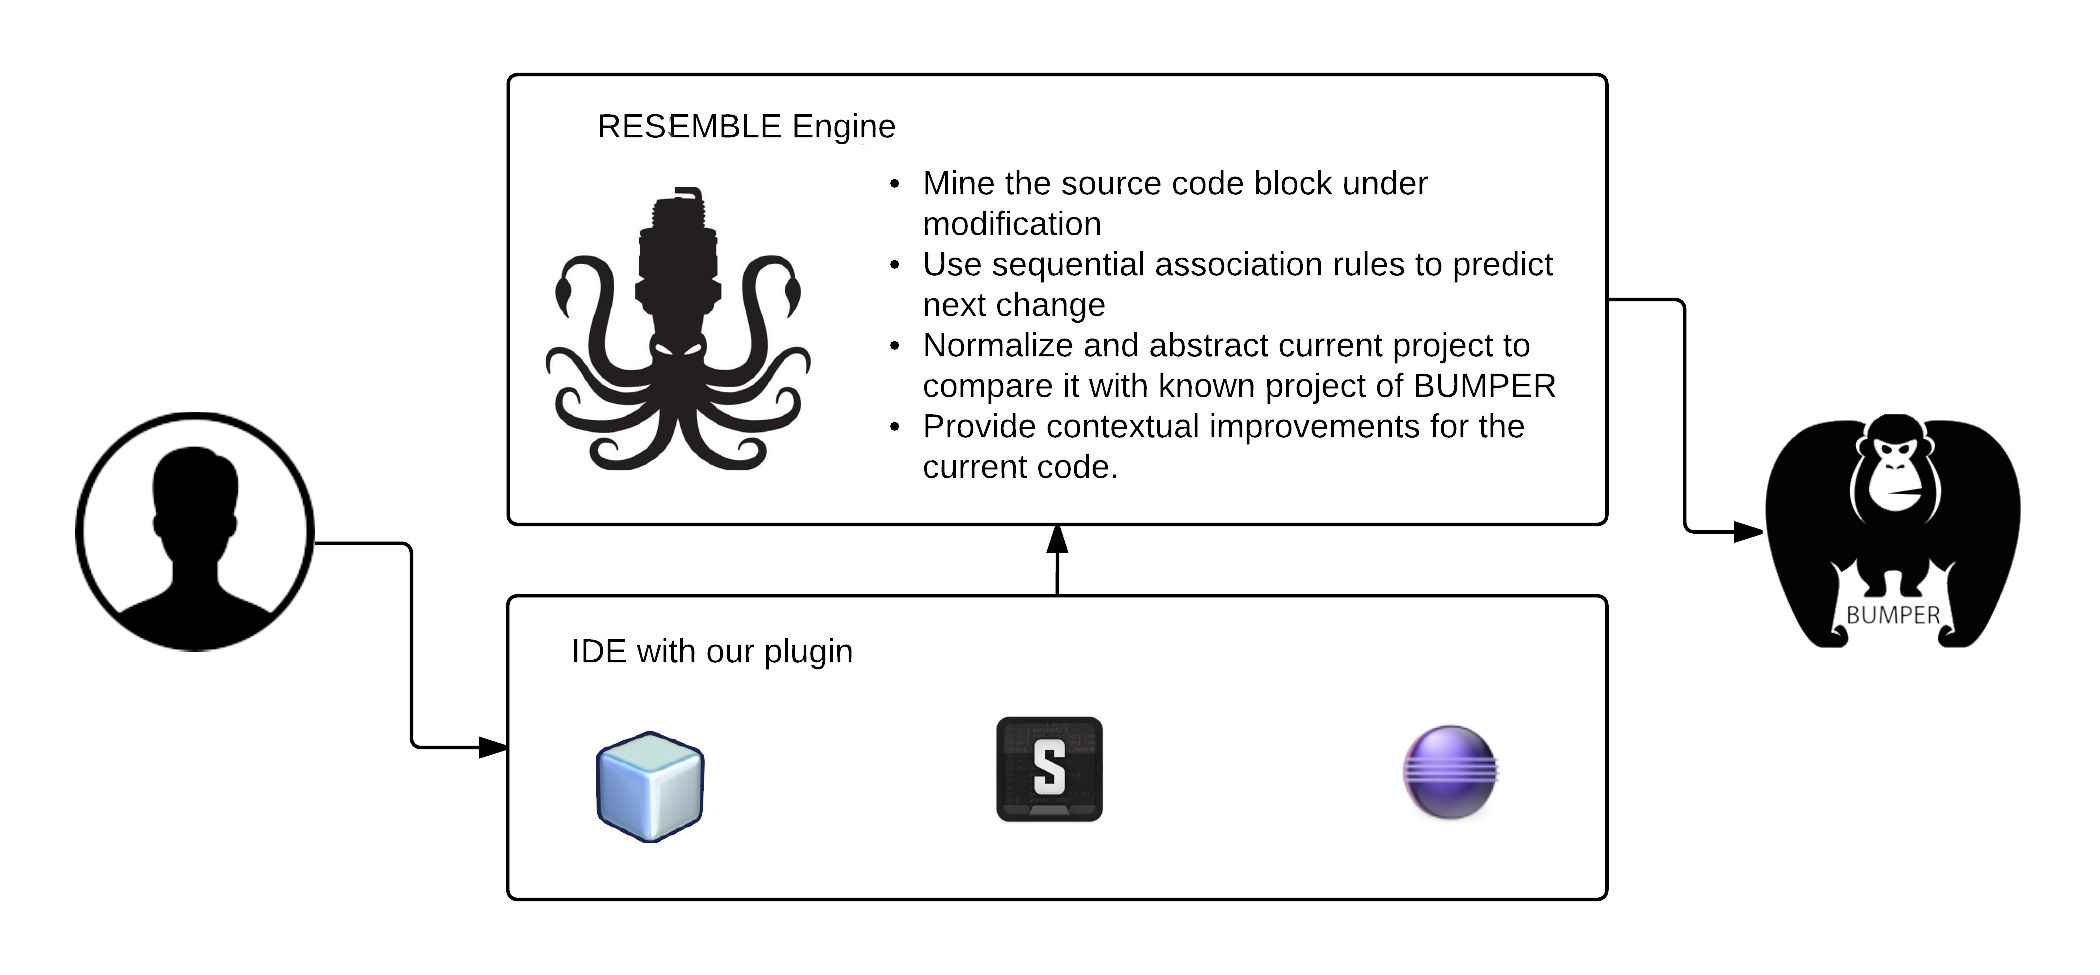
\includegraphics[scale=0.9]{media/resemble-approach.png}
    \caption{The RESEMBLE Approach
    \label{fig:RESEMBLE-approach}}
\end{figure}

In the following sections, we present the detailed steps of {\tt RESEMBLE}.

\subsubsection{Mining sequences of changes}

In the data mining field, ARM is a
well-established method for discovering co-occurrences between attributes
in the objects of a large data set \cite{Gregory1991,HEIKKI1997}. Plain
associations have the form $X \rightarrow Y$, where $X$ and $Y$,
called the \textit{antecedent} and the \textit{consequent}, respectively, are sets of descriptors
(purchases by a customer, network alarms, or any other general kind of events).
Even though plain association rules could serve some relevant information, we are interested here in
the sequences of changes that we believe will yield more precise result. Indeed, we think that similar modifications are often done in the same order by the same developer (e.g top to bottom or bottom to top).
We, therefore, adopt a variant called sequential association rules in which
both $X$ and $Y$ become sequences of descriptors.
Moreover, our sequences follow a temporal order with the antecedent preceding the consequent.
Rules of this type mined from changes reveal crucial
information about the likelihood of blocks of code to be modified together in a programming session
and, more importantly, in a specific order.
For instance, a strong rule \emph{$Block_A$ $,$ $Block_B$} implies \emph{$Block_C$} would mean that after modifying $Block_A$ and then $Block_B$, there are good chances that the developer needs to modify $Block_C$.
The conciseness of this example should not confuse the reader as in practical cases
the sequences appearing in a rule can be of an arbitrary length.
Furthermore, the strength of the rule is measured by the \textit{confidence} metric.
In probabilistic terms,
it measures the conditional probability of C appearing down the line.
Beside that, the significance of a rule, i.e. how many times it appears in the data, is provided by its \textit{support} measure.
To ensure only rules of potentially high interestingness are mined,
the mining task is tuned by minimal thresholds to
output only the sufficiently high scores for both metrics.

To extract the association rules from changes,
two choices were possible. On one hand, sequential pattern mining and rule mining algorithms
have been designed for structures that are slightly more general than the ones used here.
In fact, sequential patterns are defined on transactions that represent sequences of sets.
Efficient sequential pattern miners have been published, e.g. the PrefixSpan method \cite{Pei2004}.
On the other hand, sequence of changes do not compile to fully-blown sequential transactions as the underlying structures are mere sequences of individual elements. Such data has been known since at least the mid-90s but received less attention by the data mining community, arguably because it is less challenging to mine.
In the general data mining literature, mining from pure sequences, as opposed to sequences made of sets, has been addressed under the name of episode mining \cite{HEIKKI1997}.
Episodes are made of \textit{events} and in a sense, code changes are events. Arguably the largest body of knowledge on the subject belongs to the web usage mining field: The input data is again a system log, yet this time the log of requests sent to a web server \cite{Pei2000}.
It is noteworthy that sequential patterns are more general than the pure sequence ones, hence mining algorithms designed for the former might prove to be less efficient when applied to the latter (as additional steps might be required for listing all significant set).
Nevertheless, to jump-start our experimental study, we used a sequential pattern/rule miner that has the advantage to be freely available on the web\footnote{http://www.philippe-fournier-viger.com/spmf/}.
Although it has not been optimized for pure sequences its performances are more than satisfactory.

\subsubsection{Code Normalization\label{sec:resemble-normalization}}

Normalizing code is the action of making its structure consistent throughout the program according to a defined model. In our case, we only normalize the block of code that are in the current sequential association rules. To do so, we improve and combine several technologies such as source code transformation \cite{Cordy2006,Cordy2006a}, source code pretty-printing \cite{Roy2008}, flexible source code normalization \cite{Cordy2011}.

More specifically, the code first goes to a pretty printer. A pretty-printer is a component that will slightly transform the code in order to obtain consistent control structure.
Concretely, spaces will be added, accolade moved and tabulation added for an $if$, a $while$ and others structures to always appear the same way, regardless of the programming language.
Then, the code is normalized several times. Each normalization is different and targets specific feature of the code.
For example, we have one normalization that removes completely the variable names and replace the types by the highest known object in the object oriented hierarchy before {\tt Object} itself\footnote{For Java programs}. Another normalization only keeps the structures of the source code by normalizing both variables names and types.

\subsubsection{Comparing normalization\label{sec:resemble-comparing}}

Comparing different normalizations is the easiest step and can be done efficiently using using the longest common sequence (LCS) algorithm \cite{hirschberg1977algorithms}.
If the LCS is above an user-defined threshold, then a two different behaviors can be observed:

\begin{itemize}
	\item If the modified blocks' --- and potentially the ones that are likely to be modified after according to our sequential association rules --- normalizations match the normalizations of blocks of code that have been removed in past history. {\tt RESEMBLE} recommends the replacing code as a better solution.
  In other words, if blocks $A$, $B$ and $C$ have been replaced by blocks $A'$, $B'$ and $C'$ and blocks $D$, $E$ and $F$ normalizations match $A$, $B$ and $C$, then, {\tt RESEMBLE} recommends to transform $D$, $E$ and $F$ to look like $A'$, $B'$ and $C'$. This could lead to the introduction of software clones but we argue that (i) software clones are not always harmfull \cite{Juergens2009} and (ii) informing the developer that $A'$, $B'$ and $C'$ exist could lead him to re-use these blocks.
	\item If the modified blocks' --- and potentially of the ones that are likely to be modified after according to our sequential association rules --- normalizations match the normalization of blocks of code that are present in the history. {\tt RESEMBLE} computes the differences between the developer code and the history code in order to suggests what the developer have to do next.
\end{itemize}

\subsection{Planned experiments}

We did not started the experiments for {\tt RESEMBLE} yet as the development of the IDE plugins is not complete. Nevertheless, we plan to conduct the following experiments:

\begin{itemize}
	\item Full history test with Normalization 1.
	\item Full history test with Normalization 2.
	\item An human study where:
	\begin{itemize}
		\item Developers use {\tt RESEMBLE} in order to determine whether or not developers take into account our recommendations to avoid inserting defects in the code.
		\item Developers use {\tt RESEMBLE} in order to determine whether or not developers take into account our recommendations to complete their modification according to what we found in the history.
		\item Rate the suggested solution in a scale from 1 to 10 in order to determine if the proposed change pattern does resolve the current problem.
	\end{itemize}
\end{itemize}

We believe that {\tt RESEMBLE} will be a real asset in a developer tool belt in order to ship better code in terms of quality, performances and security.
However, as {\tt RESEMBLE} aims to provide recommendations in real-time, it will not be able to be as exhaustive as an offline process.
To fill this gap, we built {\tt BIANCA} that we present in the next section.
